% Autore= Enrico Salmaso

\subsubsection{UCS 7 - Visualizzazione della lista degli accessi di un utente riconosciuto di un'organizzazione}

\begin{figure}[h]
	\centering
	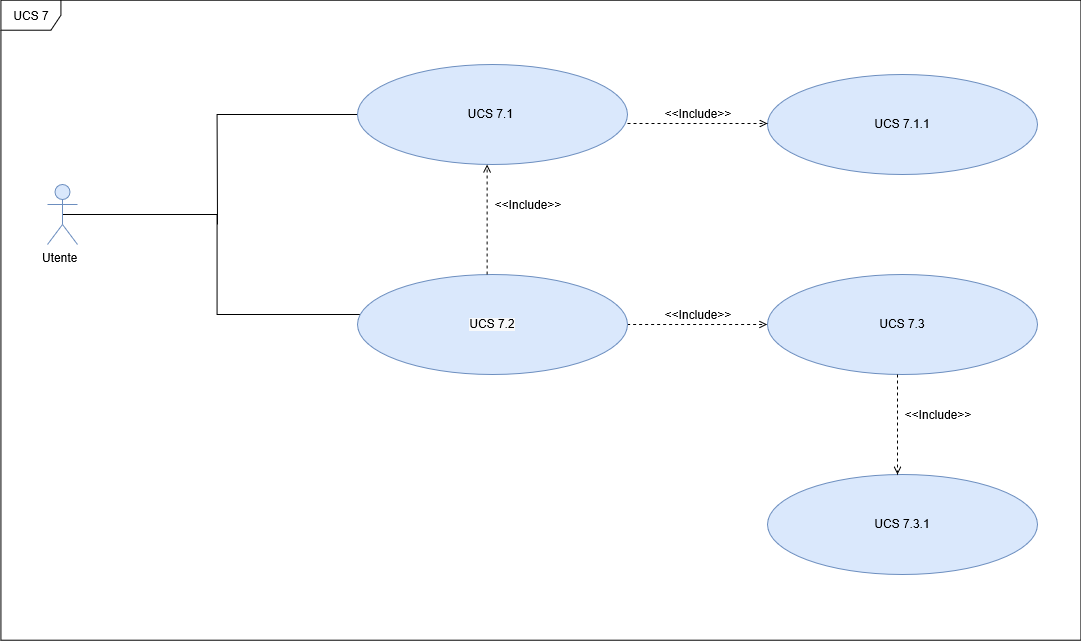
\includegraphics[scale=0.3]{sezioni/UseCase/Immagini/UCS7.png}
	\caption{UCS 7 - Visualizzazione della lista degli accessi di un utente riconosciuto di un'organizzazione}
\end{figure}

\begin{itemize}
\item \textbf{Attori primari:} Amministratore visualizzatore
\item \textbf{Precondizione:} L'amministratore deve essere autenticato presso il sistema e deve aver selezionato un'organizzazione.
\item \textbf{Postcondizione:} L'amministratore avrà visualizzato una lista di tutti gli utenti riconosciuti presenti nell'organizzazione scelta e, se vuole fare una ricerca più dettagliata, potrà selezionare la funzionalità di visualizzazione degli accessi in base a una data.
\item \textbf{Scenario principale:} L'amministratore, dopo aver selezionato l'organizzazione, accede alla funzionalità di visualizzazione della lista degli accessi per monitorare gli utenti.
\item \textbf{Flusso di eventi:} 
\begin{enumerate}
	\item L'amministratore ha selezionato l'organizzazione [UCS 3];
	\item L'amministrazione deve selezionare la funzionalità di visualizzazione della lista degli accessi.
\end{enumerate}
\item \textbf{Inclusioni:}
\begin{enumerate}
	\item UCS 3 - Selezione dell'organizzazione.
\end{enumerate}
%\item \textbf{Estensioni:} Visualizzazione di un messaggio che informa l'indisponibilità del server [?????];
\end{itemize}

\subsubsection{UCS 7.1 - Visualizzazione della lista con tutti gli utenti riconosciuti }
\begin{itemize}
	\item \textbf{Attori primari:} Amministratore visualizzatore
	\item \textbf{Precondizione:} L'amministratore si trova nella sezione di visualizzazione della lista degli accessi di un utente riconosciuto.
	\item \textbf{Postcondizione:} L'amministratore ha visualizzato la lista degli utenti riconosciuti.
	\item \textbf{Scenario principale:} L'amministratore deve aver scelto la funzionalità di visualizzazione della lista degli accessi di un utente riconosciuto per poter visualizzare tutti gli utenti riconosciuti presenti nell'organizzazione precedentemente selezionata.
	\item \textbf{Flusso di eventi:} 
	\begin{enumerate}
		\item L'amministratore visualizza tutti gli utenti riconosciuti presenti all'interno dell'organizzazione;
		\item L'amministratore selezionerà un'utente riconosciuto [UCS 7.2].
	\end{enumerate}
	\item \textbf{Inclusioni:}
	\begin{enumerate}
		\item UCS 7.2 - Selezione dell'utente riconosciuto.
	\end{enumerate}
\end{itemize}

\subsubsection{UCS 7.2 - Selezione dell'utente riconosciuto }
\begin{itemize}
\item \textbf{Attori primari:} Amministratore visualizzatore
\item \textbf{Precondizione:} L'amministratore ha visualizzato una lista con tutti gli utenti riconosciuti presenti all'interno dell'organizzazione.
\item \textbf{Postcondizione:} L'amministratore visualizzerà la lista degli accessi dell'utente riconosciuto selezionato.
\item \textbf{Scenario principale:} L'amministratore deve selezionare l'utente riconosciuto dalla lista di tutti gli utenti per poter visualizzare la sua lista degli accessi.
\item \textbf{Flusso di eventi:} 
	\begin{enumerate}
		\item L'amministratore seleziona un'utente riconosciuto dalla lista di tutti gli utenti riconosciuti presenti all'interno dell'organizzazione;
		\item L'amministratore visualizzerà tutti gli accessi dell'utente selezionato [UCS 7.3].
	\end{enumerate}
	\item \textbf{Inclusioni:}
	\begin{enumerate}
		\item UCS 7.3 - Visualizzazione degli accessi di un'utente riconosciuto.
	\end{enumerate}
\end{itemize}

\subsubsection{UCS 7.3 - Visualizzazione degli accessi di un'utente riconosciuto}
\begin{figure}[h]
	\centering
	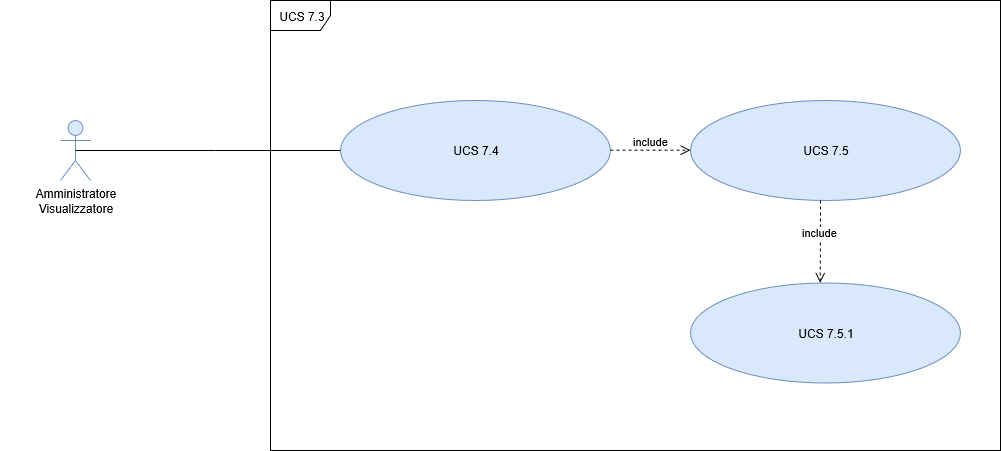
\includegraphics[scale=0.3]{sezioni/UseCase/Immagini/UCS7_1.png}
	\caption{UCS 7.3 - Visualizzazione degli accessi di un'utente riconosciuto}
\end{figure}
\begin{itemize}
	\item \textbf{Attori primari:} Amministratore visualizzatore
	\item \textbf{Precondizione:} L'amministratore ha selezionato un'utente riconosciuto.
	\item \textbf{Postcondizione:} L'amministratore avrà visualizzato una lista con gli accessi dell'utente riconosciuto selezionato e se vuole potrà approfondire la ricerca selezionando la funzionalità di visualizzazione degli accessi in base a una data.
	\item \textbf{Scenario principale:} L'amministratore ha visualizzato la lista degli accessi dell'utente riconosciuto selezionato.
	\item \textbf{Flusso di eventi:} 
	\begin{enumerate}
		\item L'amministratore visualizzerà la lista di tutti dell'utente riconosciuto;
		\item L'amministratore, se vuole, potrà selezionare la funzionalità di visualizzazione degli accessi in base a una data [UCS 7.4].
	\end{enumerate}
	\item \textbf{Inclusioni:}
	\begin{enumerate}
		\item UCS 7.4 - Selezione della funzionalità di visualizzazione degli accessi in base a una data.
	\end{enumerate}
\end{itemize}





\subsubsection{UCS 7.4 - Selezione della funzionalità di visualizzazione degli accessi in base a una data }
\begin{itemize}
	\item \textbf{Attori primari:} Amministratore visualizzatore
	\item \textbf{Precondizione:} L'amministratore avrà visualizzato tutti gli accessi dell'utente riconosciuto selezionato in precedenza.
	\item \textbf{Postcondizione:} L'amministratore potrà inserire la data per poter restringere la ricerca degli accessi.
	\item \textbf{Scenario principale:} L'amministratore, dopo aver selezionato la funzionalità di visualizzazione degli accessi in base a una data, potrà inserire una data per ottenere una ricerca più dettagliata degli accessi dell'utente riconosciuto.
	\item \textbf{Flusso di eventi:} 
	\begin{enumerate}
		\item L'amministratore ha scelto la funzionalità di visualizzazione degli accessi in base a una data;
		\item L'amministratore inserirà una data [UCS 7.5].
	\end{enumerate}
	\item \textbf{Inclusioni:}
	\begin{enumerate}
		\item UCS 7.5 - Inserimento della data.
	\end{enumerate}
\end{itemize}

\subsubsection{UCS 7.5 - Inserimento della data }
\begin{itemize}
	\item \textbf{Attori primari:} Amministratore visualizzatore
	\item \textbf{Precondizione:} L'amministratore deve aver selezionato la funzionalità di visualizzazione degli accessi in base a una data [UCS 7.4].
	\item \textbf{Postcondizione:} L'amministratore ha inserito la data.
	\item \textbf{Scenario principale:} L'amministratore, dopo aver inserito una data, potrà selezionare di visualizzare gli accessi dell'utente riconosciuto.
%	\item \textbf{Flusso di eventi:} 
%	\begin{enumerate}
%		\item L'amministratore inserisce la data in cui vuole visualizzare gli accessi di un utente riconosciuto;
%		\item L'amministratore visualizzerà gli accessi che corrispondono alla data inserita dell'utente riconosciuto precedentemente selezionato.	
%	\end{enumerate}
	%\item \textbf{Inclusioni:}
	%\begin{enumerate}
	%	\item UCS 7.5.1 - Visualizzazione degli accessi in base a una data di un'utente riconosciuto.
	%\end{enumerate}
\end{itemize}

\subsubsection{UCS 7.5.1 - Visualizzazione degli accessi in base a una data di un'utente riconosciuto }
\begin{itemize}
	\item \textbf{Attori primari:} Amministratore visualizzatore
	\item \textbf{Precondizione:} L'amministratore deve aver inserito la data.
	\item \textbf{Postcondizione:} L'amministratore avrà visualizzato una lista con gli accessi che corrispondono alla data inserita dell'utente selezionato.
\end{itemize}


